\documentclass{article}
\usepackage[utf8]{inputenc}
\usepackage{authblk}
\usepackage{setspace}
\usepackage[margin=1.25in]{geometry}
\usepackage{graphicx}
\usepackage{xcolor}
\usepackage{float}
\graphicspath{ {./figures/} }
\usepackage{amsmath,amssymb,amsfonts}
\usepackage{booktabs}
\usepackage{natbib}
\usepackage{hyperref}
\hypersetup{colorlinks=true, linkcolor=blue, citecolor=blue, urlcolor=blue}

\title{\textbf{Twelve-Minus-One Month Momentum in a Pooled Universe of Large-Cap Equities from Seven Regions}}
\author[1]{SIQuant Research}
\affil[1]{Hypothesis $\times$ Quant}
\date{\today}
\onehalfspacing

\begin{document}
\maketitle

\begin{abstract}
\noindent \textbf{Hypothesis:} $H_0$: the Sharpe ratio of past winners does not exceed that of past losers; $H_1$: it does \\
\textbf{Data:} 109 monthly cross-sections, median 126 stocks from 7 regions, 2017-09 to 2026-09 (formation months) \\
\textbf{Method:} Month-end sort on the 12-1 month cumulative return, equal-weight quintiles, one-sided stationary-bootstrap test of the Sharpe difference (5,000 draws, block 3) \\
\textbf{Results:} Sharpe 0.87 versus 0.54 (difference 0.33, one-sided $p=0.1506$); mean monthly winners-minus-losers spread 0.52\% ($t=0.70$). \\
\textbf{Research decision:} \colorbox[rgb]{0.75,0.15,0.15}{\textcolor{white}{\textbf{\,REJECTED\,}}}
\end{abstract}

\section{Design}
Momentum is the cumulative return over months $t-11$ to $t-1$, skipping the most recent month to avoid short-term reversal \citep{jegadeesh1993returns}. Stocks enter only with eleven consecutive observed months. Returns are in local currency.

\section{Results}
\begin{table}[H]
\centering
\caption{Equal-weight momentum quintiles, monthly rebalanced, local-currency returns}
\begin{tabular}{lcccc}
\toprule
Portfolio & Return & Vol & Sharpe & Max DD \\
\midrule
Winners (Q5) & 18.6\% & 22.6\% & 0.87 & -24.6\% \\
Losers (Q1) & 11.0\% & 24.7\% & 0.54 & -40.2\% \\
All stocks & 14.7\% & 15.5\% & 0.97 & -20.3\% \\
\bottomrule
\end{tabular}
\end{table}


\begin{figure}[H]
\centering
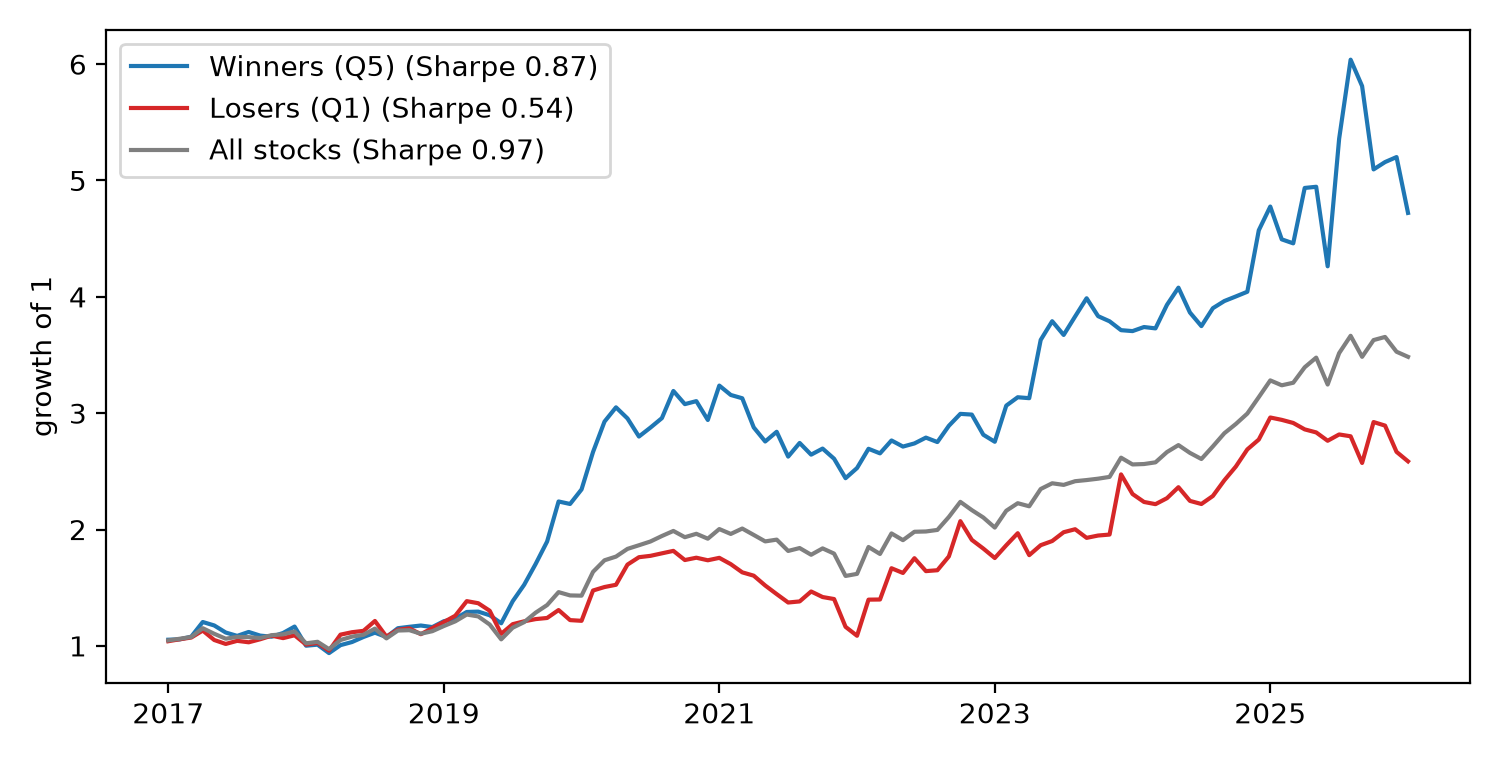
\includegraphics[width=0.8\textwidth]{fig1_momentum_quintiles.png}
\caption{Growth of one unit in the winner, loser and all-stock portfolios.}
\end{figure}

\section{Limitations}
The universe is a fixed list of today's large caps: survivorship bias helps past losers that recovered and hides delisted ones, so it works against momentum in both tails in unknown proportions. About 130 stocks give quintiles of roughly 25 names, and the decade contains a few strong momentum crashes.


\bibliographystyle{plainnat}
\bibliography{references}

\end{document}
